\chapter{Materials and Methodology}
\label{chap:methodology}

This chapter describes the data, the method and its implementation.
Section~\ref{sec:problem-formulation} presents the telecommunications dataset, analyses its categorical features and states the problem formally.
Section~\ref{sec:adopted-methodology} gives an overview of the pipeline.
The following sections describe each stage in detail: the injection of synthetic anomalies (Section~\ref{sec:anomaly-injection}), the representation of candidate hierarchies with a grammar (Section~\ref{sec:hierarchies}), the fitness function that scores a hierarchy with the \ac{MP} and the \ac{AUC} (Section~\ref{sec:fitness-evaluation}), and the configuration of the \ac{GE} search (Section~\ref{sec:ge-implementation}).
Section~\ref{sec:tools} closes the chapter with the software tools and the computational environment.

\section{Problem Formulation}
\label{sec:problem-formulation}

This research develops a hierarchical anomaly detection framework for mobile network data, with the aim of improving service reliability.
Its central question is at which level of aggregation the traffic should be monitored: a single fully aggregated series hides anomalies that affect a small segment of the traffic, while one series per combination of categorical values produces too many sparse series to monitor and interpret.
The framework answers this question with a search: candidate aggregation hierarchies are generated by a grammar, evolved with \ac{GE}, and ranked by how well a label-free detector finds known anomalies in the series they produce.

\subsection{Data Description}

The data comes from a network switch of a mobile operator and covers July to October 2022.
Each record counts the call events of one combination of categorical values in one hour, and corresponds to an aggregate of \ac{CDR}s.
The raw extract is a semicolon-separated file in which date and hour are stored in separate columns.
During preparation the two are combined into one hourly timestamp, the \#Events column is cleaned of non-numeric characters and converted to integers, the columns not used in this work (data source, date, hour and Event Duration) are dropped, and duplicated records are removed.
The resulting working dataset of 958{,}479 hourly records, spanning 2{,}110 hours from 18 July to 13 October 2022, is used throughout this dissertation.

The switch reports two metrics: \#Events, the number of call events, and Event Duration, the total call time.
Only \#Events is used as the target variable in this work, because event counts are available for both voice and SMS traffic and are the usual indicator of traffic volume.
Each record is described by six categorical features, listed in Table~\ref{tab:cdr_fields}.

\begin{table}[H]
    \centering
    \caption[Categorical features of the switch records]{Categorical features of the switch records. The letter is the symbol used for the feature in the grammar (Section~\ref{sec:grammar}).}
    \label{tab:cdr_fields}
    \begin{tabularx}{\textwidth}{llX}
        \toprule
        Letter & Feature & Description and values \\
        \midrule
        A & Call Type & Type of communication: SMS, VOICE. \\
        B & Event Type & Role of the event in the call: ORIGINATED, CALL FORWARD, TERMINATED, ROAMING OUT. \\
        C & Subscriber Type & Type of subscriber: Postpaid, Application, Roamer In, Prepaid, Other. \\
        D & Traffic Type & Destination of the traffic: OFF-NET (another operator), INT (international), ON-NET (same operator). \\
        E & Service Type & Whether the subscriber is roaming: NOT-ROAMING, ROAMING. \\
        F & Partner Description & Anonymised partner operator associated with the traffic: 392 values, P\_0001 to P\_0392. \\
        \bottomrule
    \end{tabularx}
\end{table}

Figure~\ref{fig:telecom_groups} shows the fully aggregated traffic over the whole period and Figure~\ref{fig:daily_events} zooms into eleven days of \#Events.
Both show a strong daily cycle, with low traffic at night and peaks during the day, and a weekly pattern in which weekend days differ from working days.
This regularity is what makes a shape-based detector suitable: an anomaly appears as an hour that breaks the expected daily and weekly shape.
It also motivates the window of about one week used both to inject anomalies (Section~\ref{sec:anomaly-injection}) and to compute the \ac{MP} (Section~\ref{sec:fitness-evaluation}), since one week is the shortest window that contains a complete cycle of both patterns.

\begin{figure}[H]
    \centering
    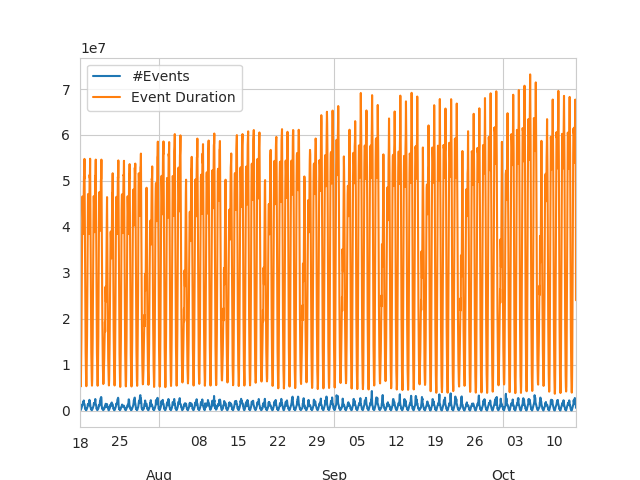
\includegraphics[scale=0.35]{figures/telecom_traffic_hierarchy.png}
    \caption[Telco network traffic metrics (\#Events and Event Duration) over July-October 2022 aggregated.]{Hourly network traffic patterns showing (A) Total \#Events (left axis) and Event Duration in hours (right axis).}
    \label{fig:telecom_groups}
\end{figure}

\begin{figure}[H]
    \centering
    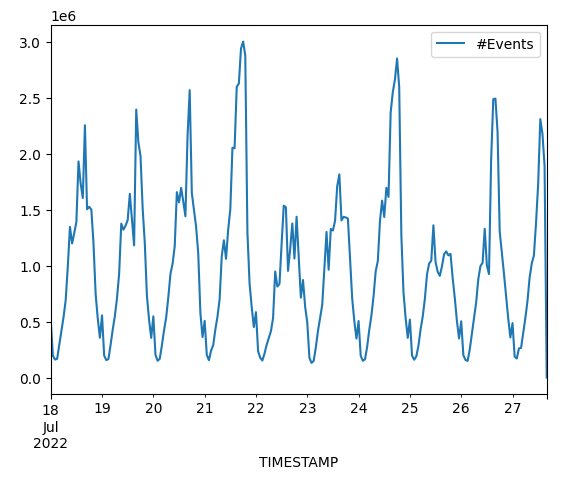
\includegraphics[scale=0.35]{figures/event_count_trend.png}
    \caption[Daily \#Events from 18--28 July 2022]{Hourly call event frequency.}
    \label{fig:daily_events}
\end{figure}

\subsection{Categorical Feature Analysis}

The six features can in theory be combined into $2 \times 4 \times 5 \times 3 \times 2 \times 392 = 94{,}080$ distinct combinations, but only 1{,}555 of them occur in the data.
Each non-empty combination is observed on average in 614 of the 2{,}110 hours of the period, with a median of only 182 hours: 94 combinations are present in every hour, while 127 appear in a single hour, so most of the corresponding series are zero for most of the time.
Table~\ref{tab:categorical_dist} describes each feature over these 1{,}555 combinations, and adds the share of the total \#Events carried by the most frequent category.

\begin{table}[H]
    \centering
    \caption[Cardinality and Dominant Categories in Telco Data]{Cardinality and Dominant Categories in Telco Data. Unique Values is the number of categories per variable; Frequency counts are out of the 1,555 non-empty feature combinations, not out of records. The last column is the share of all \#Events carried by the same top category.}
    \small
    \begin{tabular}{lrlrr}
        \toprule
        Variable & Unique Values & Top Category & Frequency & Share of \#Events \\
        \midrule
        Call Type & 2 & VOICE & 849 (54.6\%) & 45.2\% \\
        Event Type & 4 & ORIGINATED & 716 (46.0\%) & 18.3\% \\
        Subscriber Type & 5 & Roamer In & 1,486 (95.6\%) & 5.7\% \\
        Traffic Type & 3 & INT & 1,486 (95.6\%) & 21.8\% \\
        Service Type & 2 & NOT-ROAMING & 1,544 (99.3\%) & 92.4\% \\
        Partner Description & 392 & P\_0001 & 65 (4.2\%) & 94.3\% \\
        \bottomrule
    \end{tabular}
    \label{tab:categorical_dist}
\end{table}

The table reveals three distribution patterns:
\begin{itemize}
    \item \textbf{Highly skewed features.} Subscriber Type, Traffic Type and Service Type are dominated by one category in terms of combinations: 95.6\% of the combinations are Roamer In and international (INT) traffic, and 99.3\% are not roaming. Inbound roamers are associated with many different partner operators, so they generate most of the distinct combinations.
    \item \textbf{Balanced features.} Call Type (54.6\% VOICE, 45.4\% SMS) and Event Type (46.0\% ORIGINATED) split the combinations more evenly.
    \item \textbf{High-cardinality feature.} Partner Description has 392 values with a long-tail distribution; the most frequent partner appears in only 4.2\% of the combinations.
\end{itemize}

Counting combinations and counting traffic give very different pictures.
Roamer In accounts for 95.6\% of the combinations but only 5.7\% of the events: most of the traffic comes from Prepaid subscribers (63.3\% of all \#Events) and stays inside the operator's network (ON-NET, 61.3\%).
Conversely, partner P\_0001 appears in only 4.2\% of the combinations but carries 94.3\% of the events.
In other words, a few combinations carry most of the traffic, while most combinations are small and sparse.
This matters for the method: a leaf of a hierarchy that isolates a high-volume segment produces a dense, regular series, whereas a leaf that isolates a rare combination produces a sparse series that is hard to score (Section~\ref{sec:fitness-evaluation}).

The information content of each feature is measured with the Shannon entropy of its distribution over the combinations,
\begin{equation}
    H = -\sum_{i=1}^{n} p_i \log_2 p_i,
\end{equation}
where $p_i$ is the proportion of combinations with category $i$ and $n$ the number of categories.
The entropy is 0 bits when a feature takes a single value and reaches $\log_2 n$ when all values are equally frequent.
Table~\ref{tab:entropy} lists the values.

\begin{table}[H]
    \centering
    \caption[Information content by variable]{Information content by variable, computed over the 1,555 non-empty combinations. The maximum is the entropy of a uniform distribution over the same number of categories.}
    \label{tab:entropy}
    \begin{tabular}{lrr}
        \toprule
        Variable & Entropy (bits) & Maximum $\log_2 n$ (bits) \\
        \midrule
        Call Type & 0.994 & 1.000 \\
        Event Type & 1.361 & 2.000 \\
        Subscriber Type & 0.349 & 2.322 \\
        Traffic Type & 0.306 & 1.585 \\
        Service Type & 0.061 & 1.000 \\
        Partner Description & 8.404 & 8.615 \\
        \bottomrule
    \end{tabular}
\end{table}

Partner Description has by far the highest entropy (8.4 bits, close to its maximum), so splitting on it creates hundreds of branches, most of them containing very little traffic.
This has two consequences.
First, its 392 values would make the grammar and the search space much larger: every split on Partner Description would create 392 child nodes.
Second, the resulting leaves would be the sparse series on which the detector performs worst.
Partner Description is therefore excluded from the search space.
It is present in the data and in the full grammar \texttt{grammars/mobai.pybnf} (letter F), but it is dropped from \texttt{grammars/mobai\_nop.pybnf}, the grammar used in the experimental campaign.
Without it, only 77 of the $2 \times 4 \times 5 \times 3 \times 2 = 240$ possible combinations of the remaining five features occur in the data.
At the other extreme, Service Type has almost no entropy (0.06 bits): nearly all combinations are not roaming, so a split on it produces one large branch and one very small one.
It is kept in the grammar, and the search decides whether such a split is useful.

\subsection{Formal Problem Statement}
\label{sec:problem-statement}

Let each record $r$ have values $x_1(r), \dots, x_5(r)$ for the five features A--E, an hour $t(r)$, an event count $e(r)$ and an anomaly flag $a(r) \in \{0,1\}$ (Section~\ref{sec:anomaly-injection}).
A \emph{filter} $\phi$ is a conjunction of conditions of the form $x_j = v$, with at most one condition per feature, for example $\phi = (\text{Event Type} = \text{ORIGINATED}) \land (\text{Call Type} = \text{SMS})$.
Each filter defines an hourly series and its labels:
\begin{equation}
    s_\phi(t) = \sum_{r \,:\, \phi(r),\; t(r) = t} e(r),
    \qquad
    y_\phi(t) = \max_{r \,:\, \phi(r),\; t(r) = t} a(r),
    \label{eq:leaf-series}
\end{equation}
so $s_\phi(t)$ is the number of events of the matching records at hour $t$, and hour $t$ is anomalous in this series if any of these records was modified by the injection.
Hours without matching records have $s_\phi(t) = 0$ and $y_\phi(t) = 0$.

A \emph{hierarchy} $H$ is a tree whose root represents all traffic.
Each internal node splits its traffic on one feature not yet used on the path from the root, creating one child per value of that feature; each leaf $\ell$ therefore corresponds to the filter $\phi_\ell$ formed by the conditions on its path.
Because every split covers all values of the feature, the leaves of a hierarchy partition the records: each record belongs to exactly one leaf, so no traffic is lost or counted twice.
The fully aggregated series is the hierarchy with a single leaf and an empty filter.

Let $\mathcal{L}(G)$ be the set of hierarchies generated by the grammar $G$ (Section~\ref{sec:hierarchies}) and $F(H; D)$ the fitness of hierarchy $H$ on the data $D$, defined in Section~\ref{sec:fitness-evaluation}.
The problem is to find
\begin{equation}
    H^{*} = \arg\max_{H \in \mathcal{L}(G)} F(H; D_{\text{train}}),
    \label{eq:problem}
\end{equation}
the hierarchy whose leaf series allow a fixed, label-free detector to separate the injected anomalies from normal hours as well as possible on the training period.
The hierarchy found is then evaluated, without further changes, on the test period $D_{\text{test}}$.

\section{Adopted Methodology}
\label{sec:adopted-methodology}

Figure~\ref{fig:workflow} summarises the pipeline, which has five stages.

\begin{figure}[H]
    \centering
    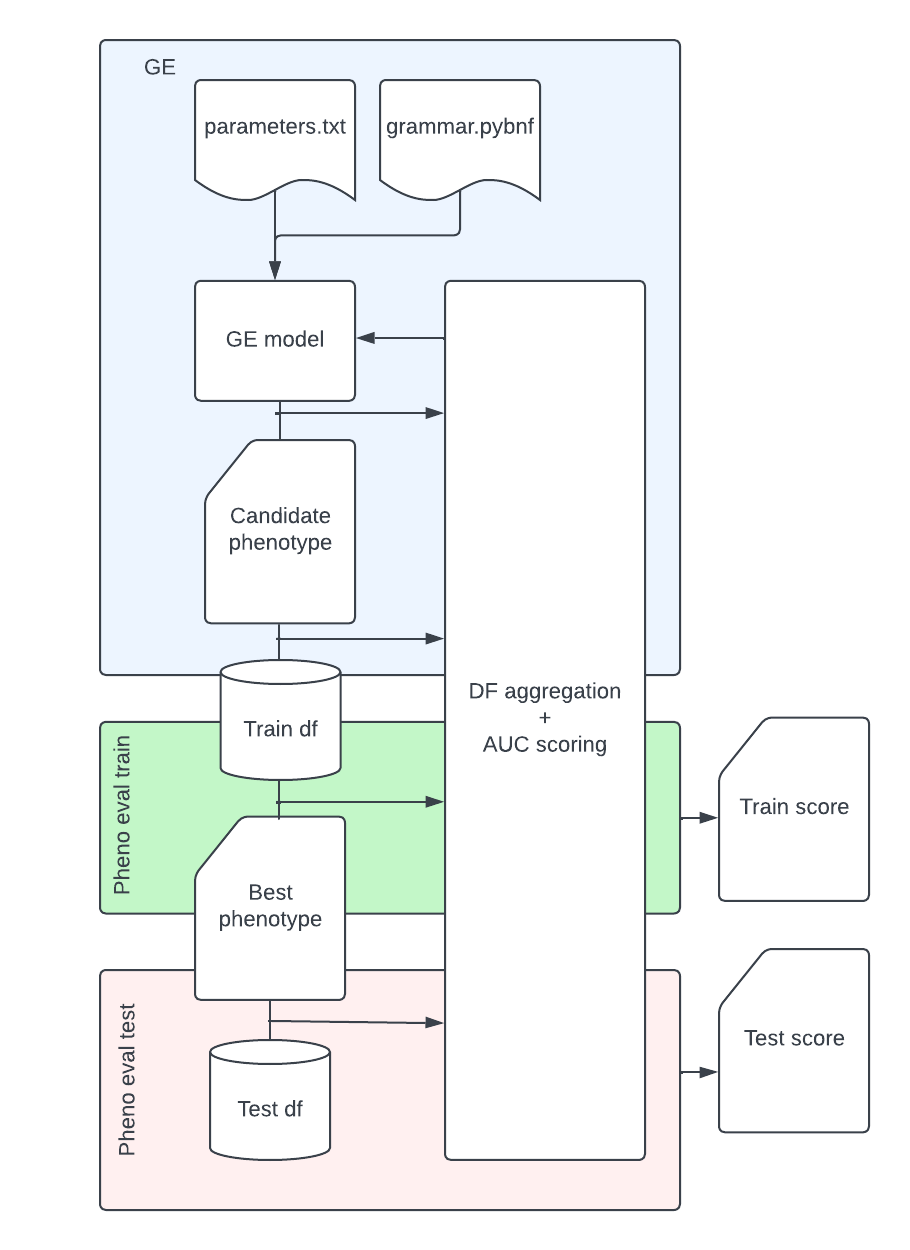
\includegraphics[scale=0.35]{figures/workflow_diagram.png}
    \caption[Anomaly detection workflow]{Hierarchical anomaly detection pipeline combining data aggregation, synthetic anomaly injection, and genetic model optimization.}
    \label{fig:workflow}
\end{figure}

\begin{enumerate}
    \item \textbf{Data preparation.}
    The raw extract is cleaned, the unused columns are dropped and duplicated records are removed, leaving 958{,}479 hourly records with six categorical features and the \#Events count.
    The records are kept disaggregated: series are built later, separately for each hierarchy, because each hierarchy defines its own aggregation.

    \item \textbf{Anomaly injection.}
    The operational data has no reliable anomaly labels, so synthetic point anomalies are inserted into 105 randomly chosen (combination, hour) pairs, one for about 5\% of the 2{,}110 hours, and the modified records are flagged (Section~\ref{sec:anomaly-injection}).
    These flags are the ground truth for the evaluation; the detector itself never sees them.

    \item \textbf{Data partitioning.}
    The data is split temporally, without shuffling, so that the test period lies entirely after the training period, as it would in operation.
    The training period runs from 18 July to 14 September 2022 (1{,}411 hours, 630{,}861 records) and the test period from 14 September to 13 October 2022 (699 hours, 327{,}618 records), roughly two thirds and one third of the data.
    The training period contains 75 anomalous hours and the test period 28.

    \item \textbf{Hierarchy search.}
    PonyGE2 evolves a population of candidate hierarchies generated by the grammar \texttt{mobai\_nop.pybnf} (Sections~\ref{sec:hierarchies} and~\ref{sec:ge-implementation}).
    Each candidate is evaluated on the training period only: its leaf series are built with Equation~\eqref{eq:leaf-series}, scored with the \ac{MP}, and compared with the anomaly flags through the weighted \ac{AUC} (Section~\ref{sec:fitness-evaluation}).

    \item \textbf{Evaluation.}
    The best hierarchy of each run is re-evaluated on the training and test periods and compared with fixed aggregation baselines (Chapter~\ref{chap:results}).
\end{enumerate}

The detector is the same in every case.
What changes from one candidate to another is only the set of series it is applied to, so differences in fitness measure the effect of the aggregation and not of the detector.

\section{Anomaly Injection}
\label{sec:anomaly-injection}

Since the operational dataset does not contain reliable anomaly labels, synthetic anomalies are injected to create a labelled evaluation scenario.
Injection has two advantages over expert labels: the position of every anomaly is known exactly, and anomalies can be placed at every level of aggregation, from the whole network to a single combination of categories.
The procedure is shown in Figures~\ref{fig:anomaly_workflow} and~\ref{alg:injection}.

\begin{figure}[htbp]
    \centering
    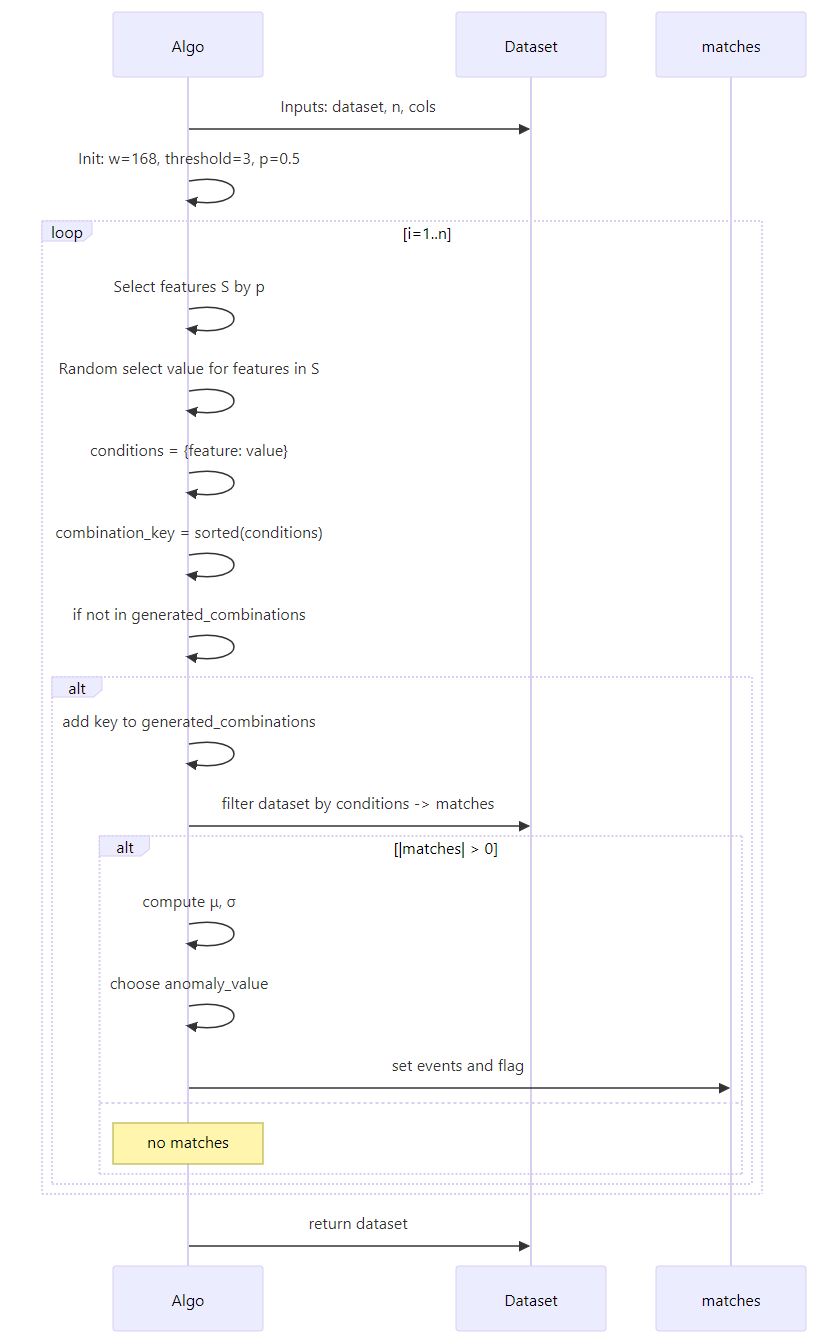
\includegraphics[height=0.75\textheight]{figures/Anomaly insertion workflow.png}
    \caption[Anomaly injection cycle]{Anomaly injection cycle.}
    \label{fig:anomaly_workflow}
\end{figure}

Each anomaly is created in four steps.
\begin{enumerate}
    \item \textbf{Choice of the affected segment.}
    Each of the six categorical features is selected independently with probability 0.5, and a value is drawn at random for each selected feature, for example $\{\text{Service Type} = \text{ROAMING}, \text{Traffic Type} = \text{INT}\}$.
    The number of conditions therefore varies: few conditions give a broad segment, such as all international traffic, and many conditions a narrow one, such as one partner for one subscriber type.
    If no feature is selected the anomaly affects all traffic.
    A combination that was already used, or that matches no records, is discarded and a new one is drawn.
    All six features are eligible, including Partner Description, so some anomalies affect segments that the grammar cannot isolate.

    \item \textbf{Choice of the hour.}
    An hour $t^{*}$ is drawn uniformly among the hours in which the segment has records.

    \item \textbf{Reference distribution.}
    The hourly \#Events series of the segment is built over the hours in which it has records, and its mean $\mu$ and standard deviation $\sigma$ are computed over a window of 167 observations around $t^{*}$ (the 84 before it, $t^{*}$ itself and the 82 after it, truncated at the ends of the series).
    For a segment present in every hour this window covers one week minus one hour and therefore a complete daily and weekly cycle; for a sparse segment, which has no records in some hours, the same number of observations spans a longer period.
    If the segment has a single observation, no window can be formed and the value is instead halved or increased by half, with equal probability.

    \item \textbf{Modification.}
    With equal probability, the anomaly is a peak or a drop.
    The new value of the segment at $t^{*}$ is $v^{*} = \mu + 3\sigma$ for a peak and $v^{*} = \max(\mu - 3\sigma, 0)$ for a drop, since an event count cannot be negative.
    The records of the segment at $t^{*}$ are rescaled by the same factor $v^{*}/s(t^{*})$, where $s(t^{*})$ is their original total, so the anomaly is distributed over the records in proportion to their original values; the new counts are rounded to integers and the records are flagged as anomalous.
\end{enumerate}

\begin{figure}[H]
    \centering
    \begin{minipage}{0.92\textwidth}
    \begin{algorithmic}[1]
        \Require records $D$, features $X_1,\dots,X_6$, number of anomalies $n$, window $w = 167$, $k = 3$
        \State $U \gets \emptyset$ \Comment{combinations already used}
        \While{fewer than $n$ anomalies have been inserted}
            \State $S \gets \{X_j : \text{a uniform random number} < 0.5\}$
            \State $\phi \gets \bigwedge_{X_j \in S} (X_j = v_j)$, with each $v_j$ drawn from the values of $X_j$
            \If{$\phi \in U$ \textbf{or} no record matches $\phi$} \textbf{continue} \EndIf
            \State $U \gets U \cup \{\phi\}$
            \State $t^{*} \gets$ hour drawn uniformly among the hours with records matching $\phi$
            \State $\mu, \sigma \gets$ mean and standard deviation of $s_\phi$ over the $w$ observations around $t^{*}$
            \State $v^{*} \gets \mu + k\sigma$ or $\max(\mu - k\sigma, 0)$, each with probability 0.5
            \For{each record $r$ with $\phi(r)$ and $t(r) = t^{*}$}
                \State $e(r) \gets \mathrm{round}\big(e(r) \cdot v^{*} / s_\phi(t^{*})\big)$; \quad $a(r) \gets 1$
            \EndFor
        \EndWhile
        \State \Return $D$
    \end{algorithmic}
    \end{minipage}
    \caption[Anomaly injection procedure]{Anomaly injection procedure.}
    \label{alg:injection}
\end{figure}

Figure~\ref{fig:anomaly_log} shows part of the log produced by the procedure.
In the first row the segment is all international traffic (Traffic Type = INT) at 08:00 on 10 September 2022: with $\mu = 234{,}009$ and $\sigma = 119{,}169$, the peak value is $\mu + 3\sigma = 591{,}516$, against an actual value of 261{,}851, so every matching record is multiplied by about 2.26.
Most of the other rows shown are drops.
For hourly traffic $\sigma$ is large relative to $\mu$, because the daily cycle alternates busy and quiet hours, so $\mu - 3\sigma$ is negative and every drop sets the segment to zero.
Drops therefore behave like outages of the segment: 30 of the 75 anomalous hours in the training period and 12 of the 28 in the test period are drops to zero, and the rest are peaks.
The 105 anomalies fall on 103 distinct hours, because in two cases the hour drawn for a new segment had already received an anomaly on another segment.

The procedure was implemented in a Kaggle notebook and executed once, without a fixed random seed.
Its output, the full record table with the modified counts and the anomaly flags, was saved and then split into the training and test sets, which are used unchanged in every run and in the final evaluation; the injected anomalies are therefore identical across all experiments, even though a new execution of the procedure would draw different ones.

\begin{figure}[htbp]
    \centering
    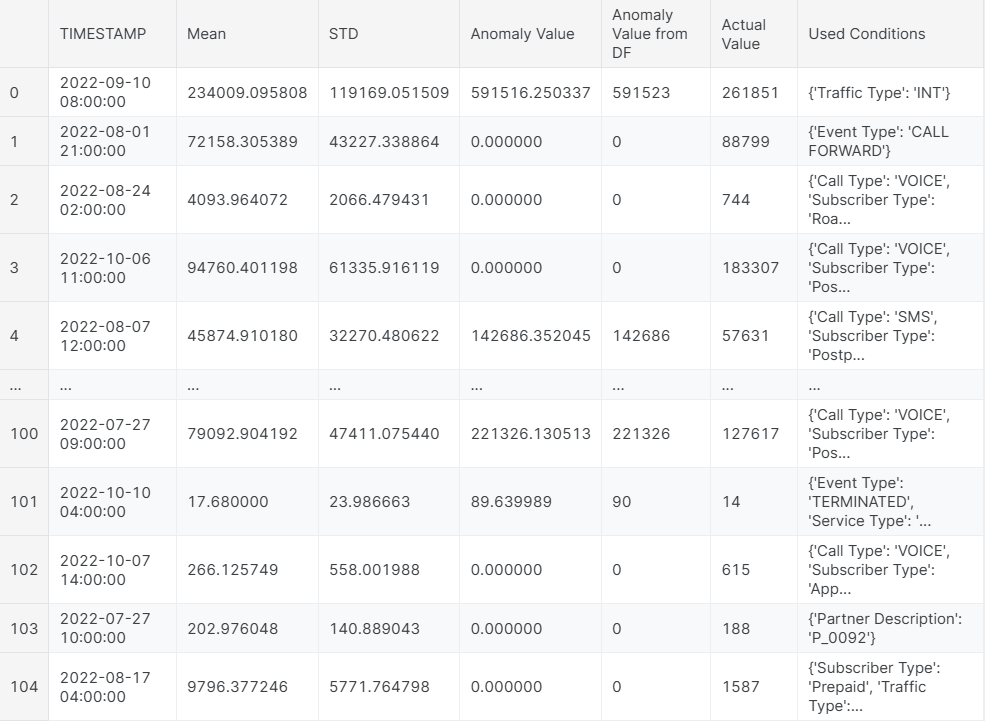
\includegraphics[width=0.95\textwidth]{figures/Anomaly log.png}
    \caption[Log of the injected anomalies]{Part of the log of injected anomalies: hour, mean and standard deviation of the segment over the reference window, target value $v^{*}$, value obtained after rounding, original value and conditions that define the segment.}
    \label{fig:anomaly_log}
\end{figure}

The window of about one week only defines the reference distribution: each anomaly is a \emph{point} anomaly that affects one hour of one segment, and the rest of the series is unchanged.
An anomaly is extreme relative to \emph{its own} segment, but it is diluted in any series that also contains other traffic.
Figure~\ref{fig:anomaly_plot} illustrates this with the two anomalies discussed above.
The peak on international traffic more than doubles that segment, but in the total traffic, of which INT is only about a fifth, the same hour lies well inside the daily range.
The drop sets CALL FORWARD events to zero, a clear outage of that segment, while the total traffic at that hour looks like an ordinary evening value.
An anomaly is easiest to detect in a series that is close to its segment, which is precisely why the choice of aggregation matters and why it is the object of the search.
Conversely, in a series that is much narrower than its segment the anomaly is spread over several leaves, each receiving the same relative change.

\begin{figure}[htbp]
    \centering
    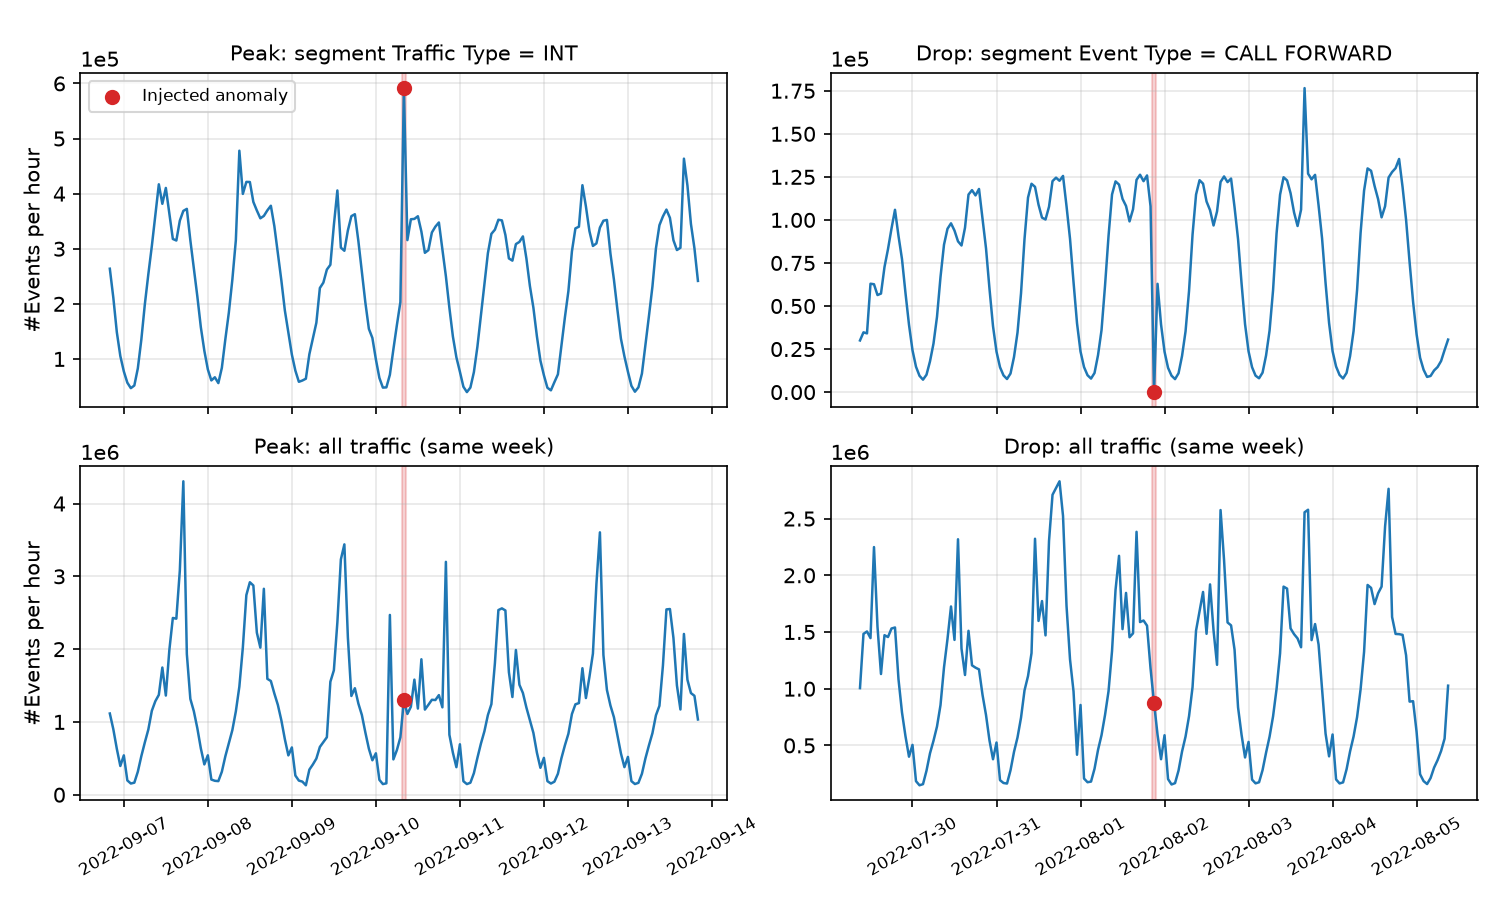
\includegraphics[width=\textwidth]{figures/injection_example.png}
    \caption[Injected anomalies on their segment and on the total traffic]{Two injected anomalies, a peak (left) and a drop (right), shown over one week on the segment that received them (top) and on the fully aggregated series (bottom). The anomalous hour is marked in red.}
    \label{fig:anomaly_plot}
\end{figure}

\section{Hierarchical Data Structures}
\label{sec:hierarchies}

There is no unique way to aggregate the data.
The same records can be monitored as one total series, as one series per call type, as one series per combination of call type and subscriber type, or by any mixture in which different branches are split on different features.
This section describes how the space of admissible hierarchies is defined with a grammar and how a hierarchy is turned into the set of series that are scored.

\subsection{Size of the Search Space}

Let $T(S)$ be the number of distinct hierarchies that can be built below a node when the features in $S$ are still unused on its path.
The node is either a leaf, or it splits on some feature $f \in S$ into $k_f$ children, each of which is again an arbitrary hierarchy over $S \setminus \{f\}$:
\begin{equation}
    T(\emptyset) = 1,
    \qquad
    T(S) = 1 + \sum_{f \in S} T(S \setminus \{f\})^{k_f}.
\end{equation}
With the five features A--E and $k_f = 2, 4, 5, 3, 2$ values, $T(\{A,\dots,E\}) \approx 2.2 \times 10^{61}$.
Exhaustive evaluation is therefore impossible, even though each hierarchy has at most 240 leaves, and the hierarchy must be found by a heuristic search.
The number of hierarchies grows so quickly because the branches of a node are independent: the traffic of one call type may be split by subscriber type while the traffic of the other call type is not split at all.

\subsection{Grammar}
\label{sec:grammar}

The admissible hierarchies are defined by the \ac{BNF} grammar \texttt{grammars/mobai\_nop.pybnf}, which has a single non-terminal \texttt{<node>}:

\begin{lstlisting}[basicstyle=\ttfamily\small, columns=fullflexible, frame=single]
<node> ::=  {:A0<node>{::}A1<node>:} |
            {:B0<node>{::}B1<node>{::}B2<node>{::}B3<node>:} |
            {:C0<node>{::}C1<node>{::}C2<node>{::}C3<node>{::}C4<node>:} |
            {:D0<node>{::}D1<node>{::}D2<node>:} |
            {:E0<node>{::}E1<node>:} |
            -END
\end{lstlisting}

Each of the first five productions splits the current node on one feature, and the last one, \texttt{-END}, makes it a leaf.
A label such as \texttt{C2} combines a letter, which identifies the feature (Table~\ref{tab:cdr_fields}), and a digit, which selects a value from that feature's list of categories in \texttt{datasets/Mobai/available\_categories.json}; for example, \texttt{C2} is Subscriber Type = Roamer In.
A split production lists \emph{all} values of its feature, each followed by a new \texttt{<node>}, so every split creates one child per value and the leaves always partition the traffic of their parent.
The symbols \texttt{\{:}, \texttt{\{::\}} and \texttt{:\}} are PonyGE2 formatting markers that open an indented block, start a new line at the same indentation and close the block.
The phenotype is therefore an indented text in which indentation encodes depth in the hierarchy, as in this excerpt of the best hierarchy evolved in the campaign (Chapter~\ref{chap:results}):

\begin{lstlisting}[basicstyle=\ttfamily\small, columns=fullflexible, frame=single]
B0
  A0-END
  A1
    C0
      C0-END
      ...
\end{lstlisting}

This fragment reads: split all traffic by Event Type; within ORIGINATED (\texttt{B0}), split by Call Type; SMS (\texttt{A0}) is a leaf; within VOICE (\texttt{A1}), split by Subscriber Type, and so on.

The grammar does not prevent a feature from being used twice on the same path, as in the second \texttt{C0} above.
Such a split is meaningless, since all the records under \texttt{C0} already have that Subscriber Type, so it is resolved when the phenotype is parsed: the branch is truncated and its parent becomes a leaf.
Keeping the grammar this simple has a cost, because part of the genetic material encodes truncated branches that do not affect the hierarchy, but it means that every derivation is a valid hierarchy and no repair or penalty is needed.
The fully aggregated series is also in the language of the grammar: it is the phenotype \texttt{-END}, a root that is a leaf.

\subsection{From Genotype to Hierarchy}

As described in Chapter~2, the genotype is a list of integer codons, and each codon selects a production with the rule $\text{codon} \bmod r$, where $r$ is the number of productions of the non-terminal being expanded.
Here \texttt{<node>} is the only non-terminal and has $r = 6$ productions, numbered 0 (split on A) to 5 (\texttt{-END}), and the non-terminals are expanded depth first, from left to right.
The genotype of the best hierarchy of the campaign starts with the codons 35341, 59028, 67535, 14390, 35960 and 29885, which map as follows:
\begin{enumerate}
    \item $35341 \bmod 6 = 1$: the root splits on B, creating \texttt{B0} to \texttt{B3}, each followed by a \texttt{<node>};
    \item $59028 \bmod 6 = 0$: the node under \texttt{B0} splits on A, creating \texttt{A0} and \texttt{A1};
    \item $67535 \bmod 6 = 5$: the node under \texttt{A0} is a leaf (\texttt{A0-END});
    \item $14390 \bmod 6 = 2$: the node under \texttt{A1} splits on C, creating \texttt{C0} to \texttt{C4};
    \item $35960 \bmod 6 = 2$: the node under \texttt{C0} splits on C again, which is later truncated;
    \item $29885 \bmod 6 = 5$: the first child of that repeated split is a leaf (\texttt{C0-END}).
\end{enumerate}
This produces exactly the excerpt shown above.
Each codon decides one node, so the number of codons used grows with the size of the hierarchy, and a derivation fails if it reaches the end of the genome before all nodes are decided (Section~\ref{sec:ge-implementation}).

\subsection{From Grammar to Series}
\label{sec:grammar-to-series}

The phenotype is parsed by \texttt{pheno\_to\_dict} (\texttt{src/fitness/mobai\_utils.py}), which reads it line by line and uses the indentation to keep track of the path from the root.
Each line adds the condition (feature, value) of its label to the path, a line ending in \texttt{END} closes a leaf, and the conditions accumulated on a root-to-leaf path become the filter of that leaf.
If a feature repeats along a path, the branch is truncated as explained above and the parent is kept as a leaf.
The output is a list of filters, one per leaf; for the excerpt above, the first two are
\begin{align*}
    \phi_1 &= \{\text{Event Type} = \text{ORIGINATED},\ \text{Call Type} = \text{SMS}\},\\
    \phi_2 &= \{\text{Event Type} = \text{ORIGINATED},\ \text{Call Type} = \text{VOICE},\ \text{Subscriber Type} = \text{Postpaid}\}.
\end{align*}

\texttt{hierarchy\_auc.evaluate} then calls \texttt{create\_final\_hierarchy}, which builds the series of Equation~\eqref{eq:leaf-series} for each leaf.
For every filter, \texttt{filter\_and\_aggregate} selects the matching records and sums \#Events and the anomaly flags per hour.
\texttt{set\_leaf} then aligns the series to the full hourly index of the split (training or test): hours with no matching records are added with \#Events $= 0$, and an hour is labelled anomalous if at least one of its records was flagged.
Alignment is needed because many segments have no records in many hours; without it, consecutive values of a series could be several hours apart and the 168-point windows of the \ac{MP} would no longer correspond to one week.

A leaf whose filter matches no records produces an empty series.
This happens often, since only 77 of the 240 combinations of the five features occur in the data.
Empty leaves carry no traffic and no anomalies, and they are ignored by the fitness function.

\section{Fitness Evaluation}
\label{sec:fitness-evaluation}

Each candidate hierarchy is evaluated by \texttt{hierarchy\_auc.evaluate}, which converts the phenotype into one hourly \#Events series per leaf (Section~\ref{sec:grammar-to-series}), scores each series with the Matrix Profile, and combines the per-leaf ROC-AUC values into a single weighted fitness.
The fitness answers the question: if an operator monitored these series with the \ac{MP}, how well would the scores rank the anomalous hours above the normal ones?

\subsection{Matrix Profile Scoring}

For each leaf series, \texttt{leaf\_scores} computes the Matrix Profile with \texttt{stumpy.stump(ts, m=168, ignore\_trivial=True)}, i.e.\ with a subsequence length of $m = 168$ hours (one week).
As explained in Chapter~2, the value of the profile at position $j$ is the z-normalised Euclidean distance between the week that starts at hour $j$ and its most similar week elsewhere in the series; trivial matches, which overlap the week itself by more than three quarters, are excluded (\texttt{ignore\_trivial}).
A high value marks a discord: a week whose shape has no close match.
The \ac{MP} needs no labels and no training, and it has a single parameter, the window length, which is fixed to one week to match the weekly cycle of the traffic.

The \ac{MP} is defined per subsequence, whereas the labels are defined per hour, so the profile has to be converted into an hourly score.
An anomaly at hour $t$ changes every week that contains $t$, that is, the 168 subsequences starting at hours $t - 167$ to $t$; the raw profile is therefore raised over a plateau of 168 positions, and does not indicate which hour of the plateau is anomalous.
The score used here is the first difference of the profile,
\begin{equation}
    \mathrm{score}(t) = P(t - m + 1) - P(t - m), \qquad t = m, \dots, N - 1,
    \label{eq:mp-score}
\end{equation}
where $P(j)$ is the profile value of the subsequence starting at hour $j$ and $N$ is the length of the series.
The subsequence starting at $t - m + 1$ is the first one whose last hour is $t$, so the score measures how much the distance increases when hour $t$ enters the window.
For an isolated anomaly this increase is largest exactly at the anomalous hour, which turns the plateau into a peak at the right position.
The scores are then min--max normalised to $[0, 1]$ within each leaf.
Since no complete window ends before hour $m$, the first 168 hours of each series are not scored and their labels are ignored: the ground truth used for the ROC-AUC is the anomaly flag from hour 168 onwards ($y_{\text{true}} = \text{Anomaly}[m{:}]$).

\subsection{Weighted AUC}

For each leaf, the \ac{ROC} \ac{AUC} measures how well the score ranks the anomalous hours above the normal hours: it is the probability that a randomly chosen anomalous hour has a higher score than a randomly chosen normal hour.
An \ac{AUC} of 1 is a perfect ranking and 0.5 is no better than random.
The \ac{AUC} does not require a detection threshold, which is convenient during the search, when no threshold has been chosen yet.

\texttt{calculate\_AUC\_hierarchy} aggregates the leaf scores.
A leaf $\ell$ is valid only if its labels after the first 168 hours contain at least two classes; let $\mathcal{L}_v$ be the set of valid leaves and $E_\ell$ the total \#Events of leaf $\ell$.
The fitness is
\begin{equation}
    F = \sum_{\ell \in \mathcal{L}_v} w_\ell \, \mathrm{AUC}_\ell,
    \qquad
    w_\ell = \frac{E_\ell}{\sum_{k \in \mathcal{L}_v} E_k},
    \label{eq:weighted-auc-ch4}
\end{equation}
where $\mathrm{AUC}_\ell$ is the ROC-AUC of the Matrix Profile score of leaf $\ell$ against its anomaly flags.

The weights reflect operational importance: a leaf that carries more traffic counts more, and a tiny leaf with a lucky \ac{AUC} cannot dominate the fitness.
They also make the fitness comparable across hierarchies with very different numbers of leaves, since the weights always sum to one.
The validity rule is necessary because the \ac{AUC} is undefined for a leaf with only one class.
Its consequence is that leaves without anomalies, including the empty ones, are excluded from the sum, so false alarms raised on them do not enter the fitness.
This limitation is discussed in Chapter~\ref{chap:results}, where a pooled \ac{AUC} that also counts these leaves is used as a robustness check.

\subsection{Evaluation Procedure}

Figure~\ref{alg:fitness} summarises the evaluation of one individual.
Individuals whose derivation fails are marked invalid by PonyGE2 before this function is called and receive no fitness (Section~\ref{sec:ge-implementation}).

\begin{figure}[H]
    \centering
    \begin{minipage}{0.92\textwidth}
    \begin{algorithmic}[1]
        \Require phenotype of an individual, training records $D_{\text{train}}$, $m = 168$
        \State $\{\phi_1, \dots, \phi_L\} \gets \texttt{pheno\_to\_dict}(\text{phenotype})$ \Comment{one filter per leaf}
        \For{$\ell = 1, \dots, L$}
            \State $s_\ell, y_\ell \gets$ hourly \#Events and labels of the records matching $\phi_\ell$, aligned to the training hours
        \EndFor
        \State $\mathcal{L}_v \gets \{\ell : y_\ell[m{:}] \text{ contains both classes}\}$
        \For{$\ell \in \mathcal{L}_v$}
            \State $P \gets \texttt{stumpy.stump}(s_\ell, m)$; \quad $\mathrm{score} \gets \text{min--max}(\mathrm{diff}(P))$
            \State $\mathrm{AUC}_\ell \gets \texttt{roc\_auc\_score}(y_\ell[m{:}], \mathrm{score})$
            \State $w_\ell \gets \sum_t s_\ell(t) \,/\, \sum_{k \in \mathcal{L}_v} \sum_t s_k(t)$
        \EndFor
        \State \Return $\sum_{\ell \in \mathcal{L}_v} w_\ell \, \mathrm{AUC}_\ell$
    \end{algorithmic}
    \end{minipage}
    \caption[Fitness evaluation of a candidate hierarchy]{Fitness evaluation of a candidate hierarchy (\texttt{hierarchy\_auc.evaluate}).}
    \label{alg:fitness}
\end{figure}

\section{Genetic Programming Implementation}
\label{sec:ge-implementation}

The genetic programming implementation is based on the PonyGE2 framework, which has the following key components:
the grammar \texttt{grammars/mobai\_nop.pybnf}, which generates candidate hierarchies over the five features A--E (Partner Description, letter F in \texttt{grammars/mobai.pybnf}, is not included);
the fitness function \texttt{hierarchy\_auc}, whose \texttt{evaluate} method calls \texttt{pheno\_to\_dict} and \texttt{create\_final\_hierarchy} to build the leaf series (Section~\ref{sec:grammar-to-series}) and \texttt{calculate\_AUC\_hierarchy} to return the weighted AUC of Equation~\eqref{eq:weighted-auc-ch4};
and the configuration parameters of Table~\ref{tab:ge-params}.
Figure~\ref{fig:ponyge2_flow} shows the control flow of PonyGE2: an initial population is generated and evaluated, and in every generation parents are selected, offspring are produced by crossover and mutation, evaluated, and replace the population.

\begin{figure}[H]
    \centering
    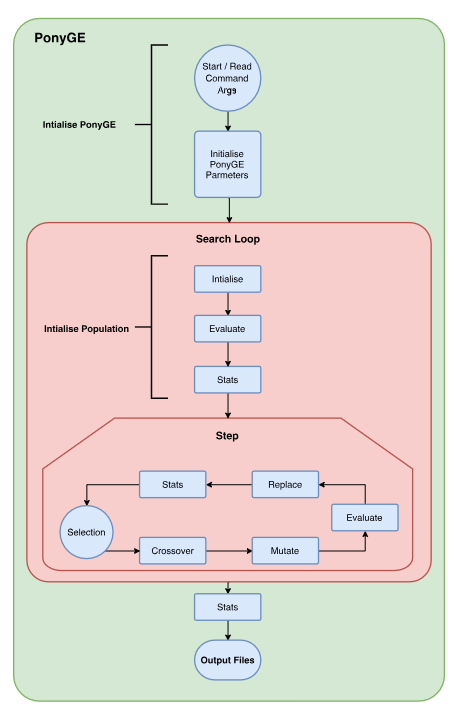
\includegraphics[scale=0.9]{figures/PonyGE2_control_flow_diagram.png}
    \caption[PonyGE2 control flow diagram.]{PonyGE2 control flow diagram \parencite{fenton2017}.}
    \label{fig:ponyge2_flow}
\end{figure}

\subsection{Genome Structure}

The genome structure is defined by codons: each codon is an integer in the range $[0, 99{,}999]$, corresponding to a codon size of 100{,}000.
Because the production is chosen with the modulo of the number of productions, which is 6 here, a large codon size makes every production equally likely for a random codon and lets mutation move freely between them.
The maximum genome length (\texttt{MAX\_GENOME\_LENGTH}) is 500 codons and represents the maximum ``DNA length'' of an individual; it prevents the genomes from growing without bound through crossover, which can produce offspring longer than their parents.
Genome wrapping is disabled (\texttt{MAX\_WRAPS} $= 0$): when a derivation needs more codons than the genome contains, the individual is invalid instead of reusing the genome from the start.
Invalid individuals receive no fitness and are not chosen as parents (\texttt{INVALID\_SELECTION} is false).

Since each codon decides one node, the length of the genome bounds the number of nodes of a hierarchy.
The largest hierarchy splits every branch on all five features, starting with the feature with most values; it has $1 + 5 + 5\cdot4 + 5\cdot4\cdot3 + 5\cdot4\cdot3\cdot2 + 240 = 446$ nodes, excluding truncated branches, and the useful hierarchies found are much smaller.
A cap of 500 codons is therefore above what such hierarchies require: it stops bloat without cutting off valid hierarchies.
The derivation depth is further limited by \texttt{MAX\_TREE\_DEPTH} $= 20$.
A useful hierarchy is at most five levels deep, since a feature repeated on a path is truncated, so this limit only constrains the truncated, non-functional branches.

\subsection{Search Operators and Parameters}

Table~\ref{tab:ge-params} lists the configuration of the experimental campaign and the role of each parameter; the operators themselves are described in Chapter~2.

\begin{table}[htbp]
    \centering
    \caption{Key Configuration Parameters (experimental campaign)}
    \label{tab:ge-params}
    \begin{tabularx}{\textwidth}{llX}
        \toprule
        Parameter & Value & Role in this work \\
        \midrule
        CODON\_SIZE & 100000 & Range of each codon, $[0, 99{,}999]$. \\
        MAX\_GENOME\_LENGTH & 500 & Upper bound on the genome; prevents bloat. \\
        MAX\_WRAPS & 0 & No wrapping: an incomplete derivation is invalid. \\
        INITIALISATION & PI\_grow & Initial trees grown in random order, at least one branch reaching the maximum initial depth. \\
        MAX\_INIT\_TREE\_DEPTH & 5 & Initial hierarchies can already use all five features. \\
        MAX\_TREE\_DEPTH & 20 & Limit on the depth of the derivation tree. \\
        POPULATION\_SIZE & 10 & Individuals per generation; small because of the cost of the fitness. \\
        GENERATIONS & 50 & Number of generations, giving 510 evaluations per run. \\
        SELECTION & tournament & Parents chosen by tournaments among random individuals. \\
        TOURNAMENT\_SIZE & 2 & Low selection pressure, which preserves diversity in a small population. \\
        CROSSOVER & variable\_onepoint & Tails of two parents swapped after independent cut points; offspring length may change. \\
        CROSSOVER\_PROBABILITY & 0.75 & Share of parent pairs that undergo crossover. \\
        MUTATION & int\_flip\_per\_codon & Each used codon replaced by a random integer with probability $1/\text{(number of used codons)}$, i.e.\ about one change per individual. \\
        REPLACEMENT & generational & The offspring replace the population in every generation. \\
        ELITE\_SIZE & 1 & The best individual is copied unchanged to the next generation. \\
        FITNESS\_FUNCTION & hierarchy\_auc & Weighted \ac{AUC} of Equation~\eqref{eq:weighted-auc-ch4} on the training period. \\
        \bottomrule
    \end{tabularx}
\end{table}

Two parameters deserve a comment.
Mutation is applied only to the used codons, that is, to the part of the genome that was read during the mapping, so every mutation changes a decision that is actually part of the hierarchy.
Because codons are read depth first, a mutation near the start of the genome changes a split close to the root and alters the meaning of all the codons that follow; a mutation near the end changes only one small branch.
The search therefore makes both large and small structural moves.
Elitism guarantees that the best fitness never decreases from one generation to the next, so the best individual of the final generation is also the best individual found in the run; this is the hierarchy reported for each run in Chapter~\ref{chap:results}.

The population size and the number of generations are much smaller than the PonyGE2 defaults and than the values in \texttt{parameters/mobai.txt} (50 and 100).
Each evaluation builds every leaf series from about 630{,}000 records and computes one \ac{MP} per valid leaf, so the budget had to be reduced to complete ten independent runs (Section~\ref{sec:tools}).
PonyGE2 caches the fitness of every phenotype already evaluated, so duplicates produced by elitism or by neutral mutations of truncated branches are not scored twice.

\section{Technological Tools and Computational Environment}
\label{sec:tools}

This section describes the technological tools used in this dissertation, the parts of the implementation that were reused and developed, and the environment in which the experimental campaign was run.
The whole pipeline, from data aggregation to the statistical tests, was implemented in Python.
This choice follows from the two core components of the method: PonyGE2 \parencite{fenton2017} and STUMPY \parencite{law2019stumpy} are both Python libraries, so the search, the scorer and the evaluation share one language and one data representation.
Table~\ref{tab:tools} lists the tools and the versions used in the experimental campaign.

\begin{table}[H]
    \centering
    \caption{Technological tools employed}
    \label{tab:tools}
    \begin{tabularx}{\textwidth}{llX}
        \toprule
        Name & Version & Role in this work \\
        \midrule
        Python & 3.13.11 & Programming language of the whole pipeline. \\
        PonyGE2 & fork & \ac{GE} engine: genotype-to-phenotype mapping through the grammar, initialisation, selection, crossover, mutation, replacement and logging of each run. \\
        STUMPY & 1.14.1 & Computation of the \ac{MP} of each leaf series with \texttt{stumpy.stump}. \\
        Numba & 0.66.0 & Just-in-time compiler used by STUMPY to run the \ac{MP} kernels as native code. \\
        pandas & 2.3.3 & Loading of the CSV datasets, filtering of the records of each leaf, hourly aggregation and alignment to the full hourly index. \\
        NumPy & 2.4.4 & Array operations, including the first difference and min--max normalisation of the \ac{MP}. \\
        scikit-learn & 1.8.0 & \ac{ROC} \ac{AUC} (\texttt{roc\_auc\_score}) and precision, recall and F1 of the pooled evaluation. \\
        SciPy & 1.17.1 & Wilcoxon signed-rank tests against the baselines. \\
        Matplotlib & 3.11.2 & Figures of Chapter~\ref{chap:results}. \\
        Kaggle Notebooks & -- & Hosted Jupyter environment used for data preparation, exploratory analysis, enumeration of the feature combinations, anomaly injection and early prototypes of the hierarchy and \ac{MP} scoring. \\
        \bottomrule
    \end{tabularx}
\end{table}

\subsection{Reused and Developed Components}

PonyGE2 is used as the search engine with its standard operators; the only changes to the framework replace the deprecated constant \texttt{np.NaN} with \texttt{np.nan} in \texttt{mapper.py} and \texttt{base\_ff.py}, which is required by NumPy~2 and does not change its behaviour.
The components specific to this problem were developed for this dissertation:
\begin{itemize}
    \item the grammar \texttt{grammars/mobai\_nop.pybnf}, which defines the space of admissible hierarchies (Section~\ref{sec:grammar});
    \item the fitness function \texttt{src/fitness/hierarchy\_auc.py}, which loads the training set once and evaluates each individual (Section~\ref{sec:fitness-evaluation});
    \item \sloppy the module \path{src/fitness/mobai_utils.py}, which parses the phenotype (\texttt{pheno\_to\_dict}), builds and aligns the leaf series (\texttt{create\_final\_hierarchy}, \texttt{set\_leaf}), scores them (\texttt{leaf\_scores}) and computes the weighted \ac{AUC} (\texttt{calculate\_AUC\_hierarchy});
    \item the script \texttt{src/evaluate\_experiment.py}, which re-evaluates the best individual of every run and the seven baselines on both periods, computes the original and pooled metrics and runs the Wilcoxon tests;
    \item the script \texttt{src/plot\_results.py}, which produces the figures and tables of Chapter~\ref{chap:results} from the saved runs.
\end{itemize}
The same functions are used during the search and in the final evaluation, so the reported test values are computed exactly as the fitness, only on the test period.

The data preparation that precedes the search was carried out in Kaggle notebooks over the private operator data.
They load the raw extract, parse the timestamps, clean the \#Events column, drop the unused columns and the duplicated records, and produce the exploratory analysis of Section~\ref{sec:problem-formulation}.
They also enumerate the 94{,}080 possible combinations of the six features and separate the 1{,}555 that occur in the data, with the number of hours in which each is observed; this list is what the injection procedure checks before accepting a segment.
Finally, they implement the anomaly injection of Section~\ref{sec:anomaly-injection} and the plots used to inspect the injected anomalies.
The same notebooks also contain the early prototypes of the approach, in which hierarchies were sampled at random and scored first with a z-score heuristic and then with the \ac{MP}; these prototypes motivated the replacement of random sampling by a grammar-guided search and are not part of the reported experiments.

\subsection{Computational Environment}

The experimental campaign was run on a desktop computer with an AMD Ryzen~7 8700F processor (8 cores, 16 threads) and 32~GB of RAM, under Windows~11.
Ten independent runs were executed, one per random seed from 0 to 9, with four runs in parallel.
Within each run, PonyGE2 evaluates the individuals of a generation on four processes (\texttt{MULTICORE}, \texttt{CORES} $= 4$) and caches the fitness of phenotypes already evaluated (\texttt{CACHE}), so duplicated individuals are not scored again.
Each run took between 13 and 20 minutes.
Most of this time is spent in the fitness function, since every evaluation filters the records and computes one \ac{MP} per leaf; this cost is the reason for the reduced population size and number of generations (Section~\ref{sec:setup}).

\subsection{Reproducibility}

Every run is identified by its random seed, and PonyGE2 stores in its result folder the full parameter file used (\texttt{parameters.txt}), the statistics of every generation (\texttt{stats.tsv}) and the best individual with its phenotype (\texttt{best.txt}).
The campaign settings (population 10, 50 generations) override the defaults of \texttt{parameters/mobai.txt}, so the stored \texttt{parameters.txt} of each run is the reference for its configuration.
\begin{sloppypar}
The final evaluation reads only these folders and the fixed training and test sets (\path{datasets/Mobai/train_set.csv} and \path{test_set.csv}), and writes the results to \texttt{evaluation.csv}, \texttt{evaluation\_pooled.csv} and \texttt{results\_tables.md}, so all values reported in Chapter~\ref{chap:results} can be regenerated without repeating the search.
\end{sloppypar}
